\documentclass{article}

\usepackage[left=2cm,right=2cm, top=2cm, bottom = 2cm]{geometry}
\usepackage{amsfonts}
%%%\usepackage{array}

\usepackage{tikz}

\pagestyle{empty}

%%%\setlength{\tabcolsep}{1.8cm}
%%%\renewcommand{\arraystretch}{2.5}

%%%\makeatletter
%%%\newcommand{\thickhline}{%
%%%    \noalign {\ifnum 0=`}\fi \hrule height 2pt
%%%    \futurelet \reserved@a \@xhline
%%%}
%%%\newcolumntype{!}{@{\hskip\tabcolsep\vrule width 2pt\hskip\tabcolsep}}
%%%\makeatother

\begin{document}

\title{Pythagoras Theorem and Trigonometric Functions}
\date{}

\maketitle

\Large

{\bf \underline{Objective: To be able to use Pythagoras Theorem and SohCahToa.}}

\vspace{5mm}


%%%%%%%%%%%
\iffalse

{\bf Recap of previous material:}

\vspace{5mm}

\begin{enumerate}
\item Solve $3x^2-8x+4=0$.
\item Find the points where the parabola with equation $y=x^2+18x-39$ meets the $x$-axis.
\item Find the points where the line $y=3x-4$ and the parabola $y=-x^2-12x+9$ intersect.
\end{enumerate}


\clearpage

\fi
%%%%%%%%%%%%




{\bf Warm-up:}

\vspace{5mm}

Consider the right-angled triangle below, with sides of length $a$, $b$, and $c$.

\begin{center}
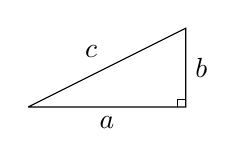
\begin{tikzpicture}
\draw (0,0) -- (2,0) -- (2,1) -- (0,0);
\draw (1.9,0) -- (1.9, 0.1) -- (2,0.1);
\node[below] at (1,0) {$a$};
\node[right] at (2,0.5) {$b$};
\node[above left] at (1,0.5) {$c$};
\end{tikzpicture}
\end{center}

Arrange two identical copies of this triangle as shown:

\begin{center}
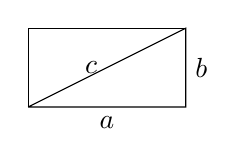
\begin{tikzpicture}
\draw (0,0) -- (2,0) -- (2,1) -- (0,0);
\node[below] at (1,0) {$a$};
\node[right] at (2,0.5) {$b$};
\node[left] at (1,0.5) {$c$};
\draw (2,1) -- (0,1) -- (0,0);
\end{tikzpicture}
\end{center}

\begin{enumerate}
\item Write an algebraic expression for the area of this rectangle.
\item Hence write an algebraic expression for the area of the triangle.
\end{enumerate}

Now arrange four identical copies of the same triangle as shown:

\begin{center}
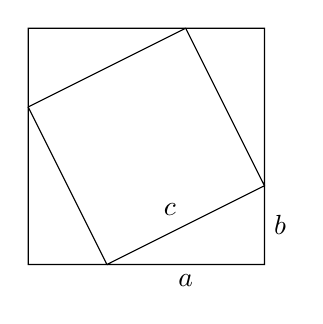
\begin{tikzpicture}
\draw (0,0) -- (2,0) -- (2,1) -- (0,0);
\node[below] at (1,0) {$a$};
\node[right] at (2,0.5) {$b$};
\node[above left] at (1,0.5) {$c$};
\draw (2,1) -- (2,3) -- (1,3) -- (2,1);
\draw (1,3) -- (-1,3) -- (-1,2) -- (1,3);
\draw (-1,2) -- (-1,0) -- (0,0) -- (-1,2);
\end{tikzpicture}
\end{center}

\begin{enumerate}
\setcounter{enumi}{2}
\item Write an algebraic expression for the area of the large square formed from these four triangles.
\item Write an algebraic expression for the area of the smaller, tilted square formed in the middle.
\item Hence write an algebraic equation relating the areas of the two squares and of the triangle.
\item Rearrange this equation to deduce Pythagoras' Theorem: $a^2+b^2=c^2$.
\item How many radians are in a circle?
\item How many radians are in $90^\circ$?
\item How many degrees are in $\pi/3$ radians?
\end{enumerate}

\clearpage


{\bf Theory - Trigonometry (SohCahToa):}

Consider the right-angled triangle below, with an angle $\theta$ labelled and sides of lengths $o$, $a$, and $h$ ({\bf o}pposite $\theta$, {\bf a}djacent to $\theta$, and the {\bf h}ypotenuse, respectively).

\begin{center}
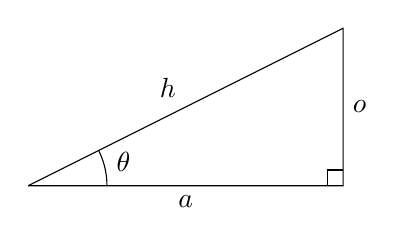
\begin{tikzpicture}
\draw (0,0) -- (4,0) -- (4,2) -- (0,0);
\draw (3.8,0) -- (3.8,0.2) -- (4,0.2);
\node[below] at (2,0) {$a$};
\node[right] at (4,1) {$o$};
\node[above left] at (2, 1) {$h$};
\draw (1,0) arc (0:26:1);
\node[right] at (1,0.3) {$\theta$};
\end{tikzpicture}
\end{center}


{\bf SOH:}

\vfill

{\bf CAH:}

\vfill

{\bf TOA:}

\vfill

\clearpage


{\bf Practice:}

\vspace{5mm}

Consider the following right-angled triangles (each to scale separately, but not with each other):

\begin{center}
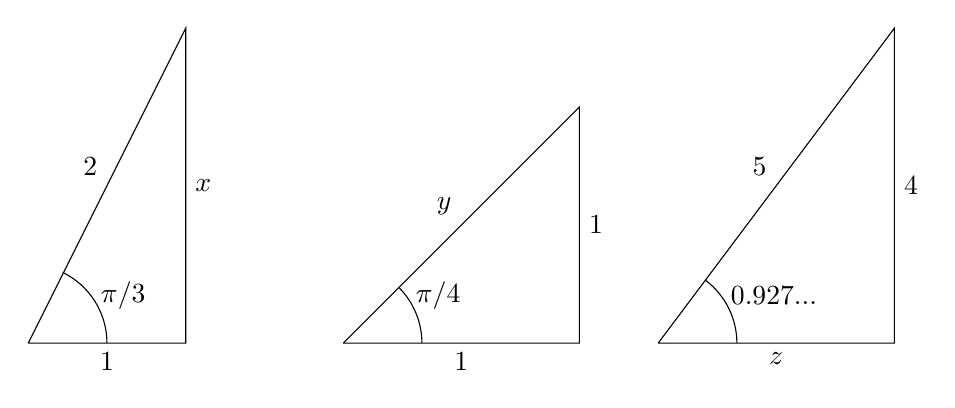
\begin{tikzpicture}
\draw(0,0) -- (2,0) -- (2,4) -- (0,0);
\node[below] at (1,0) {1};
\node[right] at (2,2) {$x$};
\node[above left] at (1,2) {$2$};
\draw (1,0) arc (0:64:1);
\node[right] at (0.8, 0.6) {$\pi/3$};

\draw (4,0) -- (7,0) -- (7,3) -- (4,0);
\node[below] at (5.5,0) {1};
\node[right] at (7,1.5) {$1$};
\node[above left] at (5.5,1.5) {$y$};
\draw (5,0) arc (0:45:1);
\node[right] at (4.8, 0.6) {$\pi/4$};

\draw (8,0) -- (11,0) -- (11,4) -- (8,0);
\node[below] at (9.5,0) {$z$};
\node[right] at (11,2) {4};
\node[above left] at (9.5,2) {5};
\draw (9,0) arc (0:53:1);
\node[right] at (8.8,0.6) {$0.927...$};
\end{tikzpicture}
\end{center}

\begin{enumerate}
\item Calcuate the missing lengths $x$, $y$, and $z$.
\item Find the areas of the 3 triangles.
\item $\sin(\pi/3)=$
\item $\cos(\pi/3)=$
\item $\sin^2(\pi/3)+\cos^2(\pi/3)=$
\item $\tan(\pi/3)=$
\item $\sin(\pi/4)=$
\item $\cos(\pi/4)=$
\item $\tan(\pi/4)=$
\item $\frac{\sin(\pi/4)}{\cos(\pi/4)}=$
\item $\tan(0.927)\approx$
\end{enumerate}

Consider again the general right-angled triangle below.

\begin{center}
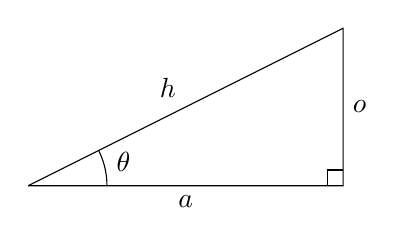
\begin{tikzpicture}
\draw (0,0) -- (4,0) -- (4,2) -- (0,0);
\draw (3.8,0) -- (3.8,0.2) -- (4,0.2);
\node[below] at (2,0) {$a$};
\node[right] at (4,1) {$o$};
\node[above left] at (2, 1) {$h$};
\draw (1,0) arc (0:26:1);
\node[right] at (1,0.3) {$\theta$};
\end{tikzpicture}
\end{center}


\begin{enumerate}
\setcounter{enumi}{9}
\item Write an expression for $\sin^2(\theta)+\cos^2(\theta)$ in terms of $o$, $a$, and $h$.
\item Simplify this expression, using Pythagoras' Theorem. Compare with question 5.
\item Express $\frac{\sin(\theta)}{\cos(\theta)}$ in terms of $o$, $a$, and $h$. Compare with question 10.
\end{enumerate}

\clearpage

{\bf Application - Angles of repose:}

\vspace{5mm}

When a granular material such as sand is poured onto a level surface, it forms a conical pile. The angle the edge of this pile makes with the ground is called the {\bf angle of repose} of the material. The angle of repose is a property of the material, and tends to be the same in different piles of the same material, even if the piles have very different sizes.

Dry sand typically has an angle of repose of around $34^\circ$ (according to Wikipedia!). If a pile of dry sand has base of radius $2m$, what is its height $h$? What is the length $l$ of the sloping side? A cross-section of the sand pile is shown below.

\begin{center}
\begin{tikzpicture}
\draw (0,0) -- (8,0) -- (4,2.7) -- (0,0);
\draw[dashed] (4,0) -- (4,2.7);
\node[above left] at (2, 1.35) {$l$};
\node[right] at (4,1.35) {$h$};
\draw[<->] (0,-0.5) -- (4,-0.5);
\node[below] at (2,-0.5) {$2m$};
\draw (1,0) arc (0:34:1);
\node[right] at (1,0.5) {$34^\circ$};
\end{tikzpicture}
\end{center}

\clearpage

{\bf Key Points to Remember:}

\vspace{5mm}

\begin{enumerate}
\item In a right-angled triangle with sides of length $a$, $b$, and $c$, where $c$ is the {\bf hypotenuse} (the longest side), {\bf Pythagoras' Theorem} states
\[a^2+b^2=c^2\]
\item If $\theta$ is an angle in a right-angled triangle ($\theta$ should not be the right angle itself), and the sides are $o$ ({\bf opposite} $\theta$), $a$ ({\bf adjacent} to $\theta$), and $h$ (the {\bf hypotenuse}), then the trigonometric functions {\bf sine}, {\bf cosine}, and {\bf tangent}, are defined by \linebreak {\bf SohCahToa}:
\[\sin(\theta)=\frac{o}{h}\qquad\qquad \cos(\theta)=\frac{a}{h}\qquad\qquad \tan(\theta) = \frac{o}{a}\]
\item For any angle $\theta$,
\[\tan(\theta)=\frac{\sin(\theta)}{\cos(\theta)}\]
\item For any angle $\theta$,
\[\sin^2(\theta)+\cos^2(\theta)=1\]
\end{enumerate}



\end{document}